% Survey of existing FPGA-based discrete event simulators, and their
% microarchitectural design.

For the purpose of this dissertation, it is insightful to classify FPGA-based
RTL simulators along two dimensions: timekeeping strategy and control
granularity. For simplicity, here we consider only single-FPGA hosts, but we
note that this discussion can trivially extended to multi-FPGA hosts. This
chapter was heavily influenced by dicussion in Pellauer and Vijayaraghavan et
al. in \emph{A-Port Networks: Preserving the Timed Behavior of Synchronous
Systems for Modeling on FPGAs}~\cite{APortNetworks}.

Timekeeping strategy refers to how the simulator tracks simulated time (target time). \emph{Explicit timekeeping}~(ET)
simulators having dedicated state to track time (in seconds) whereas simulators with implicit
timekeeping (IT) instead rely on target-cycle count as a proxy. Implicit timekeeping represents an
implementation optimization as additional FPGA resources required track and
manage timestamps are unneeded. For this optimization to apply broadly across
the simulator, in general, target clocks must have fixed frequency and phase, and
all simulation events must be synchronous to these clocks.

Control granularity refers to how time is permitted to advance across simulator. At one extreme there exist
simulators with \emph{centralized control}~(CC). These track time in
a single location: the entire simulator advances in lockstep from
timestep to timestep.  Conversely, there are simulators with \emph{distributed
control}~(DC). These simulators are parallel systems that can be represented as a directed graph of \emph{logical
processes}~(the nodes of the graph). Logical processes~(LPs) communicate by sending \emph{messages} over the graph's edges.
Each LP locally tracks simulation time and can advance independently. DC
simulators can be coarse-grained, with LPs simulating core-scale components, or
fine-grained, where LPs model blocks on the scale of CAMs, RAMs, or
combinational circuits, like multiplexers.

Taking the product of these two dimensions produces four classes of RTL simulator:

\begin{enumerate}
\item{Implicit Timekeeping, Centralized Control (ITCC)}: Simple MIDAS generated simulators~\cite{MIDAS}. FabScalar FPGA~\cite{fabscalarfpga}.

\item{Implicit Timekeeping, Distributed Control (ITDC)}: RAMP simulators~\cite{RAMPGold, HASim}, networked MIDAS-generated simulators~\cite{FireSim}.

\item{Explicit Timekeeping, Centralized Control (ETCC)}: EVE\cite{EVE}, modern commerical emulators~\footnote{As their implementations are proprietary, we can not say so definitively.}

\item{Explicit Timekeeping, Distributed Control (ETDC)}: Multi-FPGA commerical emulators~\footnote{As, above.}, This Work.
\end{enumerate}

For all intents and purposes, DC simulators are FPGA-hosted, parallel
discrete-event simulators.  Parallel, discrete-event simulation~(PDES) has been
a vibrant area of research since the 1980s, but PDES researchers have focussed
nearly exclusively on non-FPGA hosts (including multiprocessors, GPUs,
supercomputers, networks thereof).  In the next sections, we briefly introduce
relevant PDES work, and explain how prior work in that field translates to
hosting DC RTL simulators on FPGAs. First, we explore how to define simulation
peformance, and then study some CC simulator designs to help motivate the use
of DC simulators despite their increased complexity.

\section{An Iron Law For FPGA-Based Simulator Performance}

If SoC designers turn to hardware emulation for speed, it is critical
to understand how emulator design affects simulation throughput. For IT simulators with a single target-clock domain, Pellauer et al.~\cite{APortNetworks} present a simple performance
equation which, like the iron-law of processor performance that inspired it,
breaks down the performance of a complete simulation into a product of terms:

\begin{equation}
    f_{sim} = \frac{cycles_{t}}{cycles_{h}} f_{fpga}
\end{equation}\label{eq:sim-perf}

\noindent Where,
\begin{flalign*}
    f_{sim} &= \text{throughput of the simulator (target-cycles per second, Hz)}\\
    f_{fpga} &= \text{the clock frequency of the host FPGA (Hz)}\\
    cycles_{h} &= \text{the total number of host cycles over which the simulation executed}\\
    cycles_{t} &= \text{the total number of target cycles simulated}\\
\end{flalign*}

The right term of this equation, host frequency~($f_{fpga}$), is set by the
critical path delay of the simulator. Depending on the simulator's design and
the target it simulates, this may correspond to a critical path in the target design or, more frequently, a path that
drives scheduling logic in the simulator itself (i.e., some part of the circuit deciding whether to
advance forward in simulation time). The left term, a ratio of host-to-target cycles, is a measure of the
microarchitectural efficiency of the simulator. In an FPGA prototype, this term is
effectively one: every host clock simulates a target clock. In
a host-decoupled simulator, in practise, it is always less than one\footnote{While it is possible to simulate multiple target cycles per
host cycle by unrolling successive cycles of execution, there is no incentive
to do so globally across a simulator, as it would double resource utilization,
and likely double the critical path delay of the simulator. In DC simulators
of target machines with multiple clock domains, it may make sense to do this
for relatively small LPs in the fastest clock domains, if the simulator is
rate-limited on those LPs.}. Given this, Pellauer et al. tend to the
more-intuitive recipricol of this term and dubbing it the FPGA-cycles-to-Model-cycles
Ratio~(FMR). We give it in Equation~\ref{eq:fmr}. Unless it can be deduced statically,
FMR is only usefully defined over a non-trivial interval of simulation.

\begin{equation}
    FMR = \frac{cycles_{h}}{cycles_{t}}
\end{equation}\label{eq:fmr}

As an example, consider a five-read, three-write register file modelled by an LP that
uses a dual-ported BRAM. If the LP statically schedules all eight accesses, it
will have an FMR of four. Conversly, a more clever design that dynamically
schedules accesses only if the ports are used could have lower FMR: when the register file is lightly used the FMR of the LP could
approach one. Continuing with
this example, one could gang together multiple BRAMs or LUTRAMs to build a more
highly ported RAM structure capable of more port accesses per cycle~\cite{MultiportLVT, MultiportXOR}.
While this could reduce the FMR of statically scheduled implementation from four to as low as one, it
comes at the expense of FPGA resources and, potentially, a longer simulator
critical path which may counteract the FMR improvement.

To apply Equation~\ref{eq:sim-perf} to DC simulators, we can modify it to use
the FMR of the LP that has executed the fewest number of target cycles.
However, when LPs may advance only a bounded number of cycles
ahead of slower LPs in the system, for a sufficiently long simulation Equation~\ref{eq:sim-perf}
equation above returns approximately the same result for all LPs.

\section{Centrally Controlled~(CC) Simulators}

When first building a simulator, it is natural to want to coordinate time
globally across the FPGA. It is simpler to implement, there are fewer potential
sources of causality errors, and it easier to capture snapshots of the simulated system at particular points in
time. In a system where different components of the target may take differing,
or dynamically varying, number of host cycles to execute, there are two
common approaches.  The first, is what Pelleaur et al. call \emph{unit-delay
simulation}. Here the simulator is granted a fixed $N$-host-cycle budget to
compute each target cycle, where $N$ is equal the largest possible
latency a sub-block may take to execute~(i.e., in isolation its worst-case FMR is $N$). While simple to
implement, this will result in wasted host cycles as in many target cycles the
full $N$ cycle allocation may be unneeded.  We also note that while it's
relatively easy to provide tight bounds for models of many on-chip
blocks, like multi-ported RAMs, it is more difficult to do so for I/O devices, which may require large $N$
in the worst case, but far less on average.

Instead of selecting $N$ statically, a natural optimization one could make is to allow sub-blocks to signal when they have
finished computing. Here, a centralized controller aggregates done-signals from all
blocks in the system and steps the simulator only once all have been
asserted~(a wide and-reduction). This is called \emph{dynamic-barrier
synchronization}. While this removes wasted host idle-cycles (FMR can fall
below $N$), it introduces new control signals that often set the critical
path delay of the simulator: these signals must be routed to a central
location on the FPGA, propogated through a potentially wide and-reduction network, and then fanned out again across the FPGA.
This problem is exacerbated in modern FPGAs, like the VU9P devices used in EC2 F1, which are composed of multiple
dies\footnote{In Xilinx parlance, each logic die is referred to as a
super-logic regions~(SLRs).}, as these control signals must use relatively
scarser and higher-delay inter-die interconnect. Additionally, the scarcity of inter-die interconnect
puts increased pressure on the router, and for high utilizations often results
in unrouted nets, and other related DRC errors.  To improve simulator
frequency, it is natural, perhaps even necessary, to pipeline these signals at
the expense of a fixed increase to FMR: unless simulation of target cycle can
be overlapped, FMR will increase by one for each additional pipeline stage. To make things worse, while
FPGAs have scaled in capacity, their logic delays, and thus achievable
$f_{max}$, have seen little improvement. Since an increase in capacity begets
more sub-blocks, the larger and-reduction network is not offset by logic-delay
improvements which futher lengthens the critical path of the simulator.

\section{Distributed Control~(DC) Simulators}
These trends in FPGA scaling make it necessary to decentralize timekeeping to
build fast simulators.  Having more LPs, each of which manage fewer control
signals that are routed locally, improve ${f_{max}}$ while easing the routing and
DRC challenges with centralizing control. Distributing control introduces new
challenges however.  Since LPs can decouple in target time, \emph{causality errors} can
arise if LPs act on messages out of temporal order. Conversely, if LPs are too
conservative in waiting for messages to arrive the resulting simulator may be prone to deadlock.
Finally, a simulator that is correct~(it correctly models the target, and is
deadlock free), can still suffer of poor simulation performance if transmission
latency between LPs cannot be overlapped with LP execution. Designing
high-performance algorithms that satisfy these constraints for CPU hosts has been the central focus of PDES
community since its inception~\cite{PDESFujimotoPrimer}.

\subsection{A Primer on PDES}

In PDES a \emph{physical process} is divided into a set of logical processes
that communciate via timestamped messages. In effect, any one LP is it itself a discrete
event simulator that must to process events in timestamp order~(the
\emph{local causality constraint}). These events can be triggered internally or
by messages received from other LPs. The fundamental difficulty in PDES is that
an LP may not know that it has not yet received an older message and so cannot
safely being processing another event without potentially violating the local
causality constraint. A \emph{synchronization algorithm} is reponsible for
allowing LPs to make forward progress despite this. There are two broad classes of synchronization algorithm in PDES:
\emph{conservative} and \emph{optimisitic}.

In conservative synchronization algorithms, LPs wait to process events until
they are certain they will not violate the local causality constraint. This
conservatism is ripe for deadlock: it simply takes a cycle of LPs with one
waiting on the next. Conservative PDES overcomes deadlock by requiring that LPs have non-zero
\emph{lookahead}. That is to say, output messages must only depend on input
messages that are at least lookahead seconds in the past. Armed with this,
it becomes possible to detect and resolve deadlock, or avoid it altogether.
The Chandy-Misra-Bryant~(CMB)~\cite{NullMessagesBryant, NullMessagesChandy} algorithm avoids deadlock by introducing
\emph{null-messages} which indicate the absence of a real
message up to its timestamp. If an LP with non-zero lookahead, $t_{L}$, is blocked on a input whose latest
message is timestamped to time $t_{i}$, the LP must eventually issue a
null-message at time $t_{i} + t_{L}$ to each of its receivers. This may
be sufficient to unblock the receiving LP, resolving the deadlock risk. Failing that, the receiving LP is compelled to
send null-messages still further in the future and the process repeats.
So long as there exists no cycle of LPs with zero lookahead, the CMB algorithm
is garuanteed to avoid deadlock; for a complete proof we refer the interested reader to Chandy and Misra~\cite{NullMessagesChandy}.
For a given physical process, simulation performance decreases as lookahead approaches zero, as the number
of null-messages required to avoid deadlock increases~\cite{PDESFujimotoPrimer}.
In general, lookahead is derived from underlying properties of the
physical process; if sufficient lookahead cannot be
captured in the underlying system, conservative PDES algorithms may offer
little performance benefit over sequential simulators.

Optimistic synchronization algorithms, first realized by Time Warp~\cite{TimeWarp}, permit
LPs to send messages speculatively.  Here, LPs have mechanisms to rollback from
misspeculation and to inform downstream LPs of earlier messages that were
erronously sent. In Time Warp, LPs correct for mispeculated messages by
sending \emph{anti-messages}, which as the physics-analogy would suggest,
\emph{annihiliate} pair-messages that was erronously sent
in the past. In order to prevent unbounded growth of rollback state and to
gaurantee forward progress, optimistic simulators have a mechanism to determine
\emph{global virtual time}: the earliest timestamp within the set of all
unprocessed events. GVT defines a time across the entire simulator at which
the state of all LPs are known non-speculatively~\cite{TimeWarp},
rollback state before this timestamp can be reclaimed. While the most
basic conservative algorithms can be implemented more simply than optimistic
simulators, for many types of physical processes, namely those for which
sufficiently lookheads cannot be found (either deduced statically or discovered
at runtime), optimistic simulators out-perform pessimitics ones. While debate between proponents of conservative and optimistic PDES raged through
the 1990s and 2000s, both optimisitic and conservative PDES algorithms see
contemporary use~\cite{PDESRetrospective}.

%In VLSI design, optimistic VHDL and Verilog
%PDES have been built. Modern, multithreaded RTL simulators are necessarily
%PDES, though their implementation may not derive from the PDES literature. For example,
%Verilator 4.0 appears to use a form of conservative, window-based
%synchronization where it partitions a circuit into indepedent macro-tasks that
%it statically assigns to seperate threads.


\subsection{Considerations for FPGA-Hosted PDES}

FPGA differ from the multiprocessors and networked hosts studied in the PDES literature in a number of ways:

\begin{enumerate}
\item \textbf{FPGAs support bespoke, low-latency, interconnect between LPs.} Inter-LP
interconnect can be tailored for the specific simulation, producing
communication channels with very short latencies (ones of FPGA cycles).
Interconnect is relatively abundant can support hundreds or thousands
of direct links between LPs implemented on the same FPGA.

\item \textbf{FPGAs trivially support FIFO communication channels}. Unlike in
conventional PDES hosts, channels between FPGA-hosted LPs are easily made FIFO.
LPs do not need to reorder messages, and
can assume messages from the same sender arrive in monotonically increasing
time-order.

%\item \textbf{Transmissions errors are rare}. FPGA-hosted channels (i.e., hardware
%queues) operate reliably, and even those that cross asynchronously related host-clock-domains
%can be made to operate such that LPs do not need to tolerate potentially lost messages.

\item \textbf{FPGA compute resources are relatively inflexible}. FPGAs are considerably more difficult to
program as LPs and other simulation resources must be written in RTL. FPGAs lack native floating-point support which is
critical in many PDES application domains. In many cases, it is not clear that
FPGA implementation of an LP would be faster than a CPU-hosted one.
\end{enumerate}

The complexity and domain-specific knowledge required to wield FPGAs without
any gaurantee of improved performance is an enormous deterent to studying FPGAs
as hosts for general-purpose PDES. That said, at least one general-purpose, FPGA-hosted
PDES has been built: PDES-A~\cite{PDESA}. PDES-A implements an optimistic
synchronization algorithm over a regular grid of processing elements~(PEs).  While it would be
possible to implement RTL simulator using PDES-A, the effective simulation
capacity and throughput of such a system would be considerably lower than
FPGA-based emulators and prototypes. Where FPGAs hold more promise is in domain-specific PDES that
can exploit the features of its interconnect, without succumbing to the additional complexity of programming FPGAs.

\subsection{ASIC Emulation As Domain-Specific PDES}

As an application domain, ASIC emulation has a number of properties that make
FPGAs well-suited hosts. The first, most obvious reason, is that the programmability challenge is
greatly ameriolated by the fact that ASICs are already specified in RTL, and
that RTL can be efficiently mapped into an LP on an FPGA. In the case of a RTL block with a single clock, a
simple LP implementation clock-gates the block it models and adds state
machines to control when to enqueue and dequeue messages, and fire the clock.
When an LP clock fires, what would takes thousands, possibly
millions or billions, of instructions in CPU-hosted simulator is computed
concurrently in a single host cycle.

Second, since an ASIC can be decomposed into LPs, each with a relatively small,
statically defined number of neighbors, emulation can efficently leverage FPGA
interconnect. High-bandwidth interconnect between LPs removes any need to compress, or
otherwise optimize, transmission between LPs, reducing simulator complexity.
Hundreds, even thousands, of cycle-by-cycle traces of messages can be trivally
moved between LPs on the same FPGA, a feat that is all but impossible to
achieve on a CPU host. LPs can be directly connected to one another with
hardware queues, which in the general case, have a single host cycle of
"transmission" delay. In some cases, flow-through queues or wire connections
may be used to allow combinational transmission of messages.

Given that FPGAs appear to be good hosts of PDES for ASIC emulation,
the question becomes how does one translate an ASIC into a graph of
LPs, such that the resulting graph is deadlock free and preserves the behavior of the source RTL while still mapping
efficiently onto the FPGA. We refer to the set of rules that define the
behavior of these graphs as a \emph{target formalism}.
These formalisms permit building ad-hoc simulators, where a designer manually
writes LP implementations that they stitch together to model a target design
that has not yet be built~(this includes RAMPGold~\cite{RAMPGold},
HASim~\cite{HASim}, and other RAMP simulators), or hardware emulators, where
the graph is inferred by a compiler that is processing extent SoC RTL. In
the latter case, not only can LP implementations be shown to adhere to the
rules of the target formalism, but its simulated behavior can be verified
against the source RTL.

\subsection{Target Formalisms}

Target formalisms for ASIC emulation are defined by a tradeoff
between simulation performance and modeling flexibiity. More flexible
formalisms lift restrictions on LP definition and permit tighter coupling
between LPs whereas coarser-grained formalisms tend
to have better simulation performance. We explore three
formalisms: the RAMP model~(exposed as part of RDL~\cite{RDL}),
APortNetworks~\cite{APortNetworks}, and LI-BDNs~\cite{LIBDN}. One common
feature of all three formalisms is that they are designed to support conservative, ITDC
simulators: messages are not timestamped, and LPs transmit new messages to all
of their neighbors on every target cycle. When messages are not timestamped, we will refer
to them as \emph{tokens}, the term used more frequently in RAMP related works, to distingush them. 
Having a fixed-interval between tokens removes the need for conventional conservative PDES deadlock avoidance
(i.e, null messages) or detection schemes, instead deadlock avoidance in these
formalisms is acheived by-construction by constraining how combinational paths
may be modelled between LPs and the conditions under which LP implementations
must enqueue and dequeue tokens.

\subsection{Channel-Bootstrapped Formalisms}

The RAMP model~\cite{RDL} and APort Networks~\cite{APortNetworks} are examples of what we call
\emph{channel-bootstrapped} formalisms as they rely on the use of special
point-to-point LPs called \emph{channels}~(in RAMP parlance) to provide the
initial tokens of the simulation. Channels are LPs because they
model stateful interconnect: it is this statefulness that allows them to send output
tokens at time zero before receiving any input tokens.

With that said, RAMP and APortNetworks differ primarily in the granularity of
their supported non-channel LPs, or \emph{units}~(again, in RAMP parlance). The
original RAMP formalism defined units at latency-insensitive boundaries in the
target. This would make blocks on the scale of cores or DRAM controllers
reasonable candidates for definition as an LP. Channels themselves model
latency-insensitive interconnect and generically can be defined by four
parameters as shown in Figure~\ref{fig:queue-channel}.

\begin{figure}[htb]
    \centering
    \begin{subfigure}[t]{0.65\textwidth}
        \captionsetup{margin=0.25cm}
        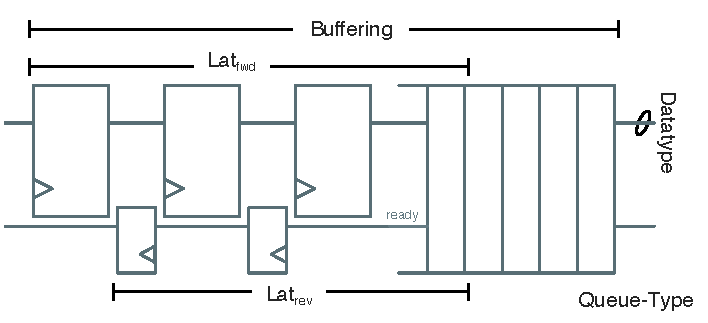
\includegraphics[width=\columnwidth]{figures/queue-channel.pdf}
        \caption{A queue type channel with its four characteristic parameters.}
        % graffle2pdf -c queue midas-graphics/graffle/channel-types.graffle figures/queue-channel.pdf
        \label{fig:queue-channel}
    \end{subfigure}
    \begin{subfigure}[t]{0.34\textwidth}
        \captionsetup{margin=0.25cm}
        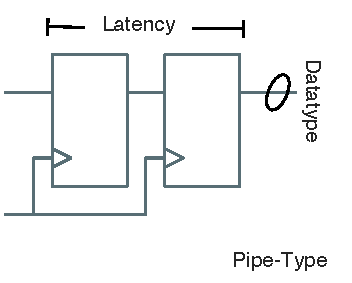
\includegraphics[width=\columnwidth]{figures/pipe-channel.pdf}
        \caption{A pipe-type channel. Setting latency to zero models a wire.}
        % graffle2pdf -c pipe midas-graphics/graffle/channel-types.graffle figures/pipe-channel.pdf
        \label{fig:pipe-channel}
    \end{subfigure}
    \centering
    \caption{Two types of channels used in a channel-bootstrapped formalism.}
\end{figure}

In practise, it is rare to find boundaries in the target where all
interfaces are latency insensitive, as often some subset of signals, like reset
and interrupts, are driven combinationally or through a set of register stages.
APort Networks~\cite{APortNetworks} was designed to support
finer-grained LPs that are coupled in this fashion. In their
paper, Pelleaur et al. use a processor pipeline as a motivating example and
divide different pipeline stages into seperate LPs. Later versions of the RAMP
architecture introduced the same sort of channel, which we call a \emph{pipe}
channel, shown in Figure~\ref{fig:pipe-channel}.  Pipe channels are defined by
a single parameter $l$, corresponding to their latency. Assuming the underlying
registers the channel models are not reset explicitly a using target signal, but are
instead initialized at time zero to some statically known value, pipe channels
provide $l$ initial tokens before they must wait for an input token.

Neither formalism appears to give any treatment to modeling a target-driven reset in
channels, as they both rely on time-zero intialization to effectively
"reset" target state.  We note that if these underlying state elements are
synchronously reset, the channels with $l >= 1$ may provide no more than one
initial token, as future tokens may causually depend on a reset
token\footnote{We further note that neither of these formalisms was designed
to support asynchronously reset as all-events are synchronous to an implicit
clock. Asynchronous reset mandates that that even
the first token emitted by a pipe-channel with $l > 0$ would depend causually
on reset at time zero.}. A pipe-type channel with $l = 0$, is a degenerate LP
that models a wire between the producer and consumer LP, coupling them
combinationally. Wire-type channels model no target state and merely relays tokens from producer to consumer.

In both formalisms, units simulate a single target cycle of execution by dequeuing an input token
from each of its input ports, and enqueing a new output token into each of
its output ports. The simplest unit implementation, and the one perscribed by
APort Networks, waits for all input tokens to arrive and all of its output
ports to be ready to accept to tokens, before it may fire. Then the
unit computes its state updates and simulateously enqueues a single output
token into each output port, and dequeues a token from each input port.
Figure~\ref{fig:adder-example} demonstrates the execution of a two target cycles in a channel-bootstrapped formalism.

\begin{figure}
    \centering
    \begin{subfigure}[t]{0.49\textwidth}
        \captionsetup{margin=0.25cm}
        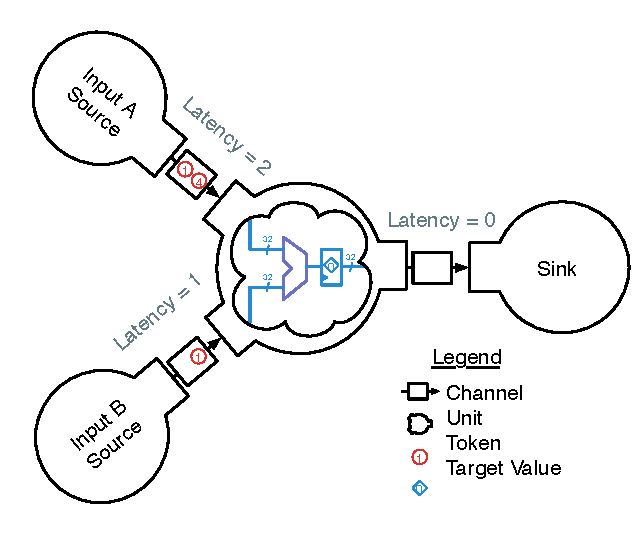
\includegraphics[width=\columnwidth]{figures/adder-example1.pdf}
        \caption{Initial state of the graph.}
        % graffle2pdf -c initial-state midas-graphics/graffle/adder-example.graffle figures/adder-example1.pdf
    \end{subfigure}
    \begin{subfigure}[t]{0.49\textwidth}
        \captionsetup{margin=0.25cm}
        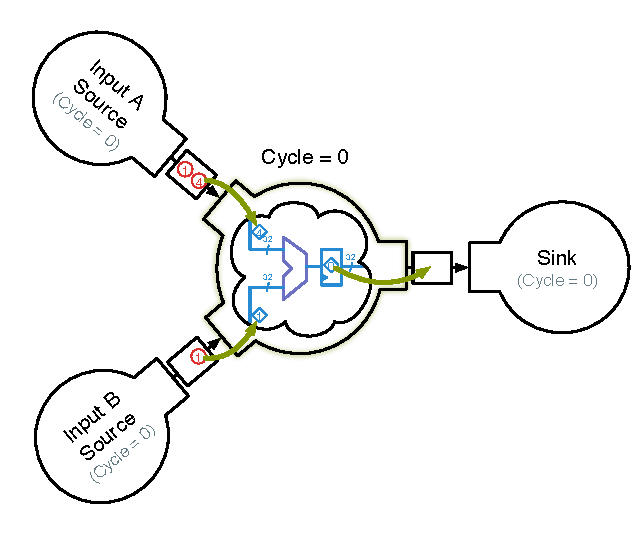
\includegraphics[width=\columnwidth]{figures/adder-example2.pdf}
        \caption{With all input tokens available, the unit fires and advances to cycle 1.}
        % graffle2pdf -c tfire-cycle0 midas-graphics/graffle/adder-example.graffle figures/adder-example2.pdf
    \end{subfigure}
    \begin{subfigure}[t]{0.49\textwidth}
        \captionsetup{margin=0.25cm}
        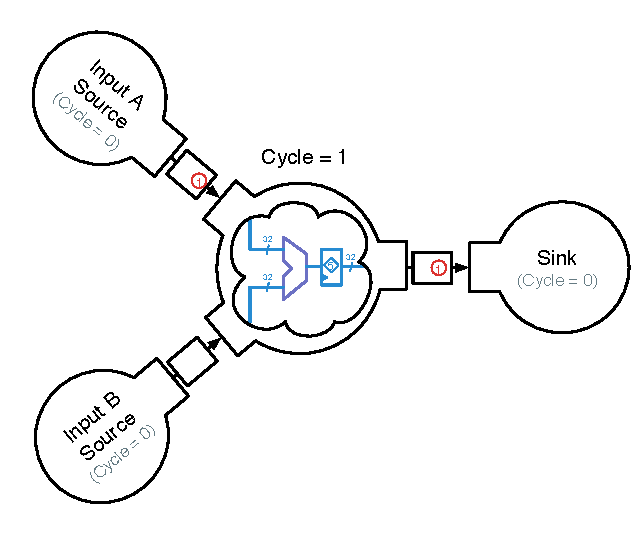
\includegraphics[width=\columnwidth]{figures/adder-example3.pdf}
        \caption{The state of the graph after firing. The unit is stalled on the arrival of a B-input token.}
        % graffle2pdf -c cycle1 midas-graphics/graffle/adder-example.graffle figures/adder-example3.pdf
    \end{subfigure}
    \begin{subfigure}[t]{0.49\textwidth}
        \captionsetup{margin=0.25cm}
        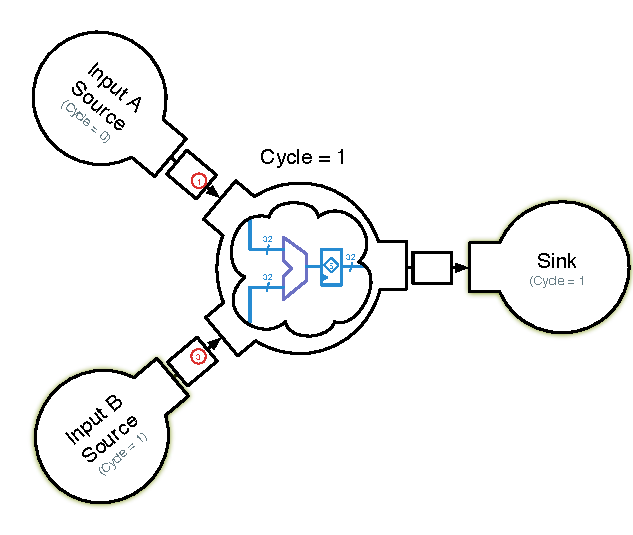
\includegraphics[width=\columnwidth]{figures/adder-example4.pdf}
        \caption{Input B source fires, producing the needed token.}
        % graffle2pdf -c inputb-fires midas-graphics/graffle/adder-example.graffle figures/adder-example4.pdf
    \end{subfigure}
    \begin{subfigure}[t]{0.49\textwidth}
        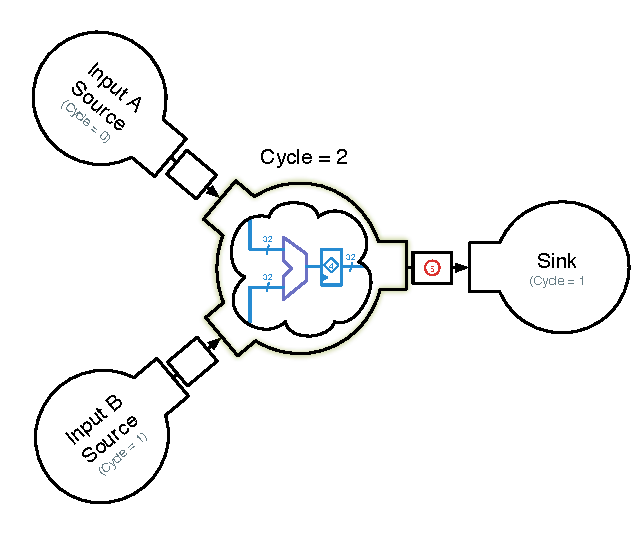
\includegraphics[width=\columnwidth]{figures/adder-example5.pdf}
        \caption{The state of the graph after two firings of the unit.}
        % graffle2pdf -c cycle2 midas-graphics/graffle/adder-example.graffle figures/adder-example5.pdf
    \end{subfigure}
    \centering
    \caption{A 32-bit adder model and environment simulating two cycles of target time.}
    \label{fig:adder-example}
\end{figure}

If the simulation designer uses exclusively non-wire-type channels, both
formalisms are free of deadlock as there exists no unit whose output at cycle
$t$ depends on the output of another unit also at cycle $t$\footnote{From a
conservative PDES persective, every LP has a non-zero lookahead, and given that
all LPs send tokens at every timestamp (obviating the need for null
messages) deadlock is avoided by construction}. In these simulators, all units
can excute cycle $t$ concurrently which, assuming no other sources of delay,
permits the simulator to run at unity FMR.  As is the case with latency-insensitive boundaries, it is not always possible to define LPs
at registered boundaries.  The use of wire-type channels (i.e. combinational
coupling between LPs) introduces two principle challenges: at best it
increases simulator FMR, and at worst it may introduce time-zero simulation
deadlock. To illustrate each of these effects, in Figure~\ref{fig:channel-deadlock} we consider a
latency-insensitive interface between two units implemented three different ways: with a queue-type
channel, with one pipe and one wire-type channel, and with two wire-type channels.

\begin{figure}
    \centering
    \begin{subfigure}[t]{0.49\textwidth}
        \captionsetup{margin=0.25cm}
        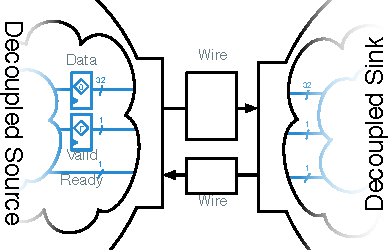
\includegraphics[width=\columnwidth]{figures/li-wire-channel-manual.pdf}
        \caption{Two-wire type channels. This deadlocks an APort Network, as neither producer nor consumer unit can fire
        before the other.}
        % -c wire midas-graphics/graffle/deadlock.graffle figures/li-wire-channel.pdf
    \end{subfigure}
    \begin{subfigure}[t]{0.49\textwidth}
        \captionsetup{margin=0.25cm}
        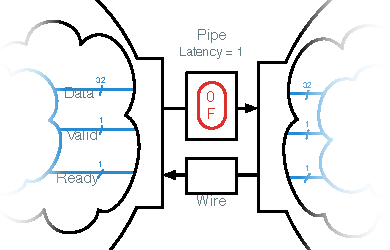
\includegraphics[width=\columnwidth]{figures/li-pipe-channel-manual.pdf}
        \caption{One pipe-type channel, and one-wire type channel carrying the backpressure. This leads $FMR >= 2$, with the consumer unit
        firing first to produce a backpressure token that is subsequently consumed by the producer unit.}
        %  -c pipe midas-graphics/graffle/deadlock.graffle figures/li-pipe-channel.pdf
    \end{subfigure}
    \begin{subfigure}[t]{0.49\textwidth}
        \captionsetup{margin=0.25cm}
        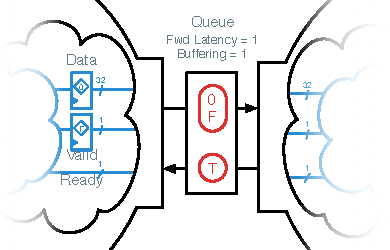
\includegraphics[width=\columnwidth]{figures/li-queue-channel-manual.pdf}
        \caption{A queue-type channel. This allows both models to
        fire simultaenously, but may only be used if it is acceptable to model
        a target queue in the channel.}
        %  -c queue midas-graphics/graffle/deadlock.graffle figures/li-queue-channel.pdf
    \end{subfigure}
    \centering
    \caption{Three potential channel modelling decisions for a latency insensitive interface between two units.}
    \label{fig:channel-deadlock}
\end{figure}

In the absence of deadlock wire-type channels tend to increase FMR as in
general a combinational path that spans $N$, units will take $N$ cycles to
execute. Note that other channels connecting these units tends to prevent
pipelining multiple cycles of target execution (i.e., this latency cannot be
overlapped, with the simulation of younger target cycles).

Deadlock is the more pressing challenge. Wire-type channels remove the
aforementioned property that all LPs have non-zero lookahead.  Here there are
two situations that may emerge. If the target itself has a combinational loop,
the behavior of the physical system is itself undefined, and simulation
deadlock is unavoidable~\footnote{We note it is possible to have "false"
combinational loops but many tools reject these patterns, and so it's not
unreasonable to ban them in these simulators as well.}. As a matter of
practise, hardware designers know to avoid combinational loops. The second
challenge arises from poor LP implementation, such as the implementation perscribed by
APort Networks, that attempts to enqueue and dequeue multiple tokens
simultaenously. Mandating this implementation has the effect of introducing a
dependency between all output tokens on all input tokens, even though there
they may be no combinational path between them in
the underlying target. Given its definition of a unit, APort Networks do not
give the correct set of constraints to avoid deadlock as a graph that contains
a cycle of wire-type channels -- that do \emph{not} represent a combinational loop in
the target -- deadlocks at time zero.


\subsection{Latency-Insensitive Bounded-Dataflow Networks~(LI-BDN)}

Unlike channel bootstrapped formalisms, LI-BDNs avoid deadlock by imposing
different constraints on the implementation of LPs based on the underlying
hardware they model, and remove the need for specialized channels to bootstrap
simulation. Since connections between LPs always represent wire-like
connectivity, LI-BDNs impose no contraints on how a synchronous target
is divided into LPs. LI-BDNs were originally developed as a more flexible abstraction for building
latency-sensitive designs that preserve the RTL timing of a synchronous circuit, extending
the work of Carloni et al., in the Theory of Latency Insensitive Design~\cite{TheoryOfLIDesign}, however the authors identify that this problem is analogous
to constructing an ITDC simulator from synchronous ASIC RTL.

In the terms of Vijayaraghavan et al.\cite{LIBDN}, what we have loosely referred to as a synchronous
block of RTL thus far is defined synchronous sequential machine~(SSM). Vijayaraghavan et
al.\cite{LIBDN} formally define an SSM:

\begin{widequote}
An SSM is a network of combinational operators or gates
such as AND, OR, NOT, and state elements such as registers,
provided the network does not contain any cycles which has
only combinational elements.
\end{widequote}

Missing from this definition is any treatment of multiple clock domains, different
types of state elements, asynchronous set or reset.  Inherent to the name
``synchronous'', Vijayaraghavan et al. forbid their existence -- in an SSM
\emph{all} state updates occur simultaenously. While this limits the
applicability of their approach, much of a modern SoC, such as the islands of a
GALS-based design, locally meets this definition.  With its simple
state-update semantics, any SSM can be easily converted into a \emph{patient
SSM}: the equivalent circuit whose state update can be controlled with the
assertion of a global enable signal.
One way this conversion can be achieved, proposed by the authors, is by
disabling register updates and masking off RAM write-enables when this control
signal is unset. Alternatively, we note that the SSM may be clock-gated.

With an SSM defined, we can now define an LI-BDN, and how they can be used to implement any
SSM in an latency-insensitive manner. An LI-BDN is a dataflow network of latency-insensitive nodes whose
edges represent FIFO communication channels with non-zero, but finite capacity. The latency-insensitive nodes of the graph are
referred to as \emph{Primitive LI-BDNs}~(in PDES terms, these are LPs), which is to say, they 
are not themselves subgraphs of more than one node. A
LI-BDN is said to \emph{implement} an SSM, if it \emph{partially implements}
the SSM, and is deadlock free. In the terms of a hardware engineer, partial implementation~(PI) implies that
the token trace of outputs from the ports of the LI-BDN "matches" the
per-cycle trace of outputs from the SSM. Vijayaraghavan et al.\cite{LIBDN}
formally define PI:

\begin{widequote}
A BDN $R$ partially implements an SSM $S$ iff
\begin{enumerate}
\item There is a bijective mapping between the inputs of $S$ and
[the input tokens of] $R$, and a bijective mapping between the outputs of $S$ and
[the output tokens of] $R$.
\item The output histories of $S$ and $R$ match whenever the
input histories match, i.e.,
\begin{align*}
\forall n &> 0\\
&\text{$I(k)$ for $S$ and $R$ matches $(1 \leq k \leq n)$}\\
\Rightarrow &\text{$O(j)$ for $S$ and $R$ matches $(1 \leq j \leq n)$}
\end{align*}
\end{enumerate}
\end{widequote}

All SSMs have infinitely many possible partial implementations~\footnote{For
instance, one can take any existing partial implementation, and introduce an
extra cycle of delay on any of its outputs. As we'll show later, since it's
always possible to produce an LI-BDN from any SSM, it follows by induction that are infinitely many partial implementations
for any SSM.}, though some implementations deadlock when composed into larger graphs.
Consider the unit implementation perscribed by APort Networks: it produces valid partial implementations of
source RTL, however it cannot implement a larger SSM when it is composed
with other liked-styled implementations without the use of non-wire-type channels (which are in essence LPs that remove zero-cycle loops between units).
Conversly, LI-BDNs garauntee deadlock freedom by adhering to two additional properties.
The first is \emph{no extraenous depedencies}~(NED) which defines when an LP is obligated to enqueue output tokens. Vijayaraghavan et al.\cite{LIBDN} formally define NED:

\begin{widequote}
A primitive BDN has the NED property if all output FIFOs have been enqueued at least $n-1$ times,
and for each output $O_i$, all the FIFOs for the inputs in $\emph{CombinationallyConnected}(O_i)$
are enqueued $n$ times, and all other input FIFOs are enqueued at least $n-1$ times, then $O_i$ FIFO
must eventually be enqueued $n$ times.
\end{widequote}\label{def:ned}

One intuitive explanation of NED is that it exploits the same observation that
permits a pipe-type channel to send output tokens before receiving any input
tokens: any output driven only by state in the LP (i.e., outputs not
combinationally coupled to an input) can enqueue an output tokens for cycle
$t$ before receiving any input tokens for cycle $t$. NED broadens this to apply to logic cones fed not just by state
elements but those that depend only on a subset of the LP's inputs.

The second property an LI-BDN must satisfy is the \emph{self-cleaning}~(SC) property. SC 
defines when an LP is obligated to dequeue input tokens. Vijayaraghavan et al.\cite{LIBDN} formally define SC:

\begin{widequote}
A primitive BDN has the SC property, if when all the
outputs are enqueued $n$ times, all the input FIFOs must
[eventually]\footnote{Clarified in~\cite{LIBDNMasters}.} be dequeued $n$ times, assuming an infinite source for each
input.
\end{widequote}\label{def:sc}

While the nodes of an APort Network do not always satisfy NED, they do satisfy
SC. At its heart, SC provides an assurance that LPs drain their input FIFOs,
allowing those FIFOs to have a bounded size. We note that if an LP fails to satisfy
SC, it will likely fail to partially implement its SSM unless its outputs are
completely independent of the inputs from which it is failing to dequeue. In
this case having unbounded FIFOs would suffice to prevent deadlock.

Of particular concern to this dissertation is a method through which an SSM can
be converted into a primitive LI-BDN.  Vijayaraghavan et al. describe a means
that uses a wrapper module around a patient SSM: a modified version of proposed wrapper circuit, for a
single output, is shown in Figure~\ref{fig:libdn-wrapper}. In contrast, we show an equivalent wrapper
circuit for an APort Network unit in Figure~\ref{fig:aport-network-wrapper}.
The LI-BDN wrapper adds one bit of state per output port~(\texttt{OFired}). The logic cone that drives
\texttt{CycleFinishing} is fed by these registers in addition to the same signals that feed
\texttt{targetFire} in the APortNetwork wrapper and so will have greater logic delay. The wrapper circuit
suggested by Vijayaraghavan et al. drives \texttt{CycleFinishing} with the and-reduction of all \texttt{OFired}
registers -- this reduces logic delay at expense of increasing FMR by 1. Conversly, both wrapper
circuits in Figures~\ref{fig:libdn-wrapper, fig:aport-network-wrapper} can run at unity FMR.
We note that both wrapper circuits are highly amenable to automatic generation with a FAME compiler.
In addition to the ability to translate an SSM into a patient SSM, the LI-BDN wrapper requires
need only a mechanism to analyze combinational depedencies in the underlying SSM.

\begin{figure}
    \centering
    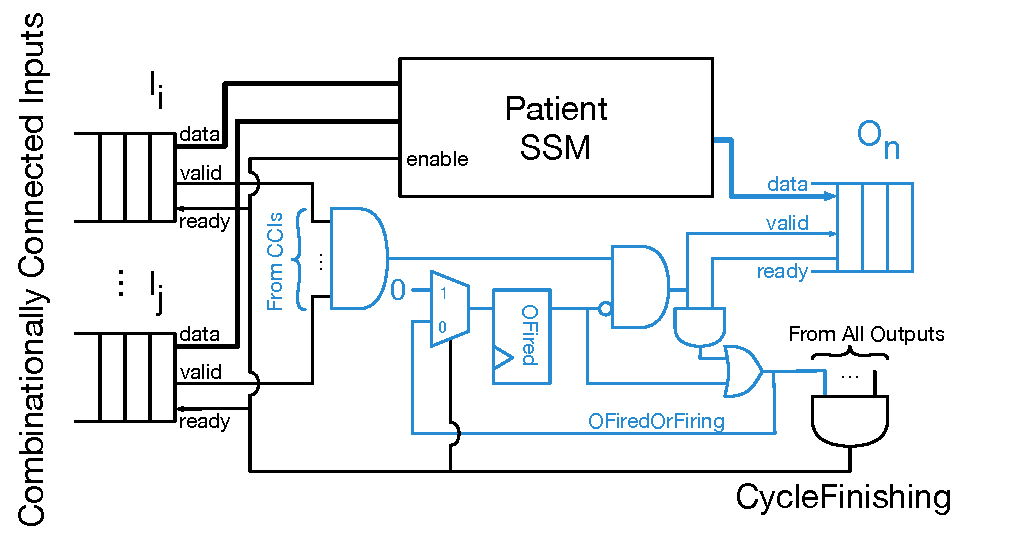
\includegraphics[width=0.99\textwidth]{figures/libdn-wrapper.pdf}
    % graffle2pdf -c libdn-wrapper midas-graphics/graffle/wrapper-transforms.graffle figures/libdn-wrapper.pdf
    \caption{A wrapper-module-based conversion of a patient SSM into a primitive LI-BDN. The logic in blue
    is generated per-output, whereas logic in black is instantiated once.}
    \label{fig:libdn-wrapper}
\end{figure}

\begin{figure}
    \centering
    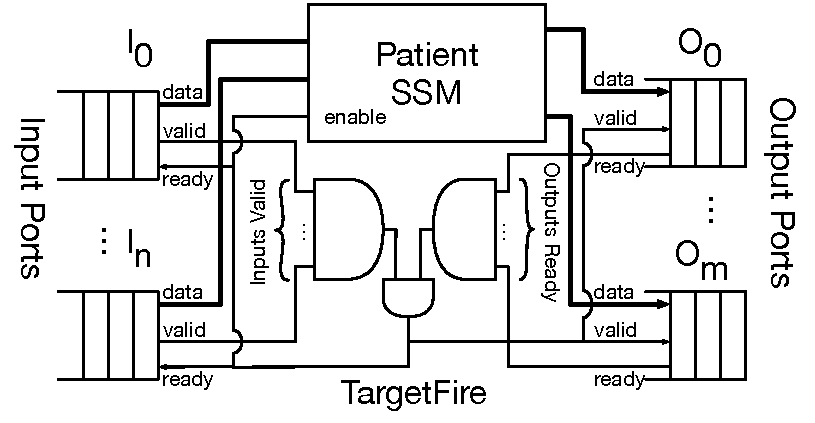
\includegraphics[width=0.9\textwidth]{figures/aport-network-wrapper.pdf}
    % graffle2pdf -c aport-network-wrapper midas-graphics/graffle/wrapper-transforms.graffle figures/aport-network-wrapper.pdf
    \caption{A wrapper-module-based conversion of a patient SSM into an APort Network unit.}
    \label{fig:aport-network-wrapper}
\end{figure}

\section{The MIDAS Compiler \& Simulator Microarchitecture}
Up to now, As we first introduce in Section~\ref{sec:midas-intro} mentioned previously,
MIDAS was our first attempt at building a FAME compiler. Here we describe the
version of MIDAS released with FireSim 1.5.0, which differs modestly from earlier iterations 
described in the CARRV paper~\cite{MIDAS} and Donggyu Kim's dissertation~\cite{DGKDissertation}.

MIDAS generates ITDC simulators from directly ASIC RTL. These simulators that
implement a channel-bootstrapped formalism, with all target graphs having a
star topology. We show an example graph for a Rocket-Chip-based system, the
most commonly used target generator in MIDAS, in Figure~\ref{fig:rocket-target-graph}.
"hub" unit is transformed from ASIC RTL elaborated by a user-provided Chisel
generator. This RTL does not represent a
closed system -- it exposes I/O interfaces that must be tied to units that model those
devices. These units are called \emph{endpoints} and form satelite nodes in the graph.
MIDAS-generated simulators are designed to run on hybrid CPU-FPGA hosts
with the expectation being that certain tightly coupled endpoints, such a DRAM
timing models, will be written in RTL and hosted on the FPGA, while other higher
latency, less performance critical ones, such UART and block device models, can
be written in software hosted on the CPU. We refer to the CPU-hosted componenet
of the simulator as the \emph{driver}. To avoid deadlock and provide good
simulation FMR, MIDAS injects queue-type channels (to model a 2-deep,
fully-decoupled FIFO) on all decoupled interfaces, and 1-cycle-latency
pipe-type channels. Assuming units do not stall internally, MIDAS-generated
simulators can run at unity FMR. We show an example simulator mapped to an EC2 F1 host in Figure~\ref{fig:mapped-simulator-f1}.

\begin{figure}
    \centering
    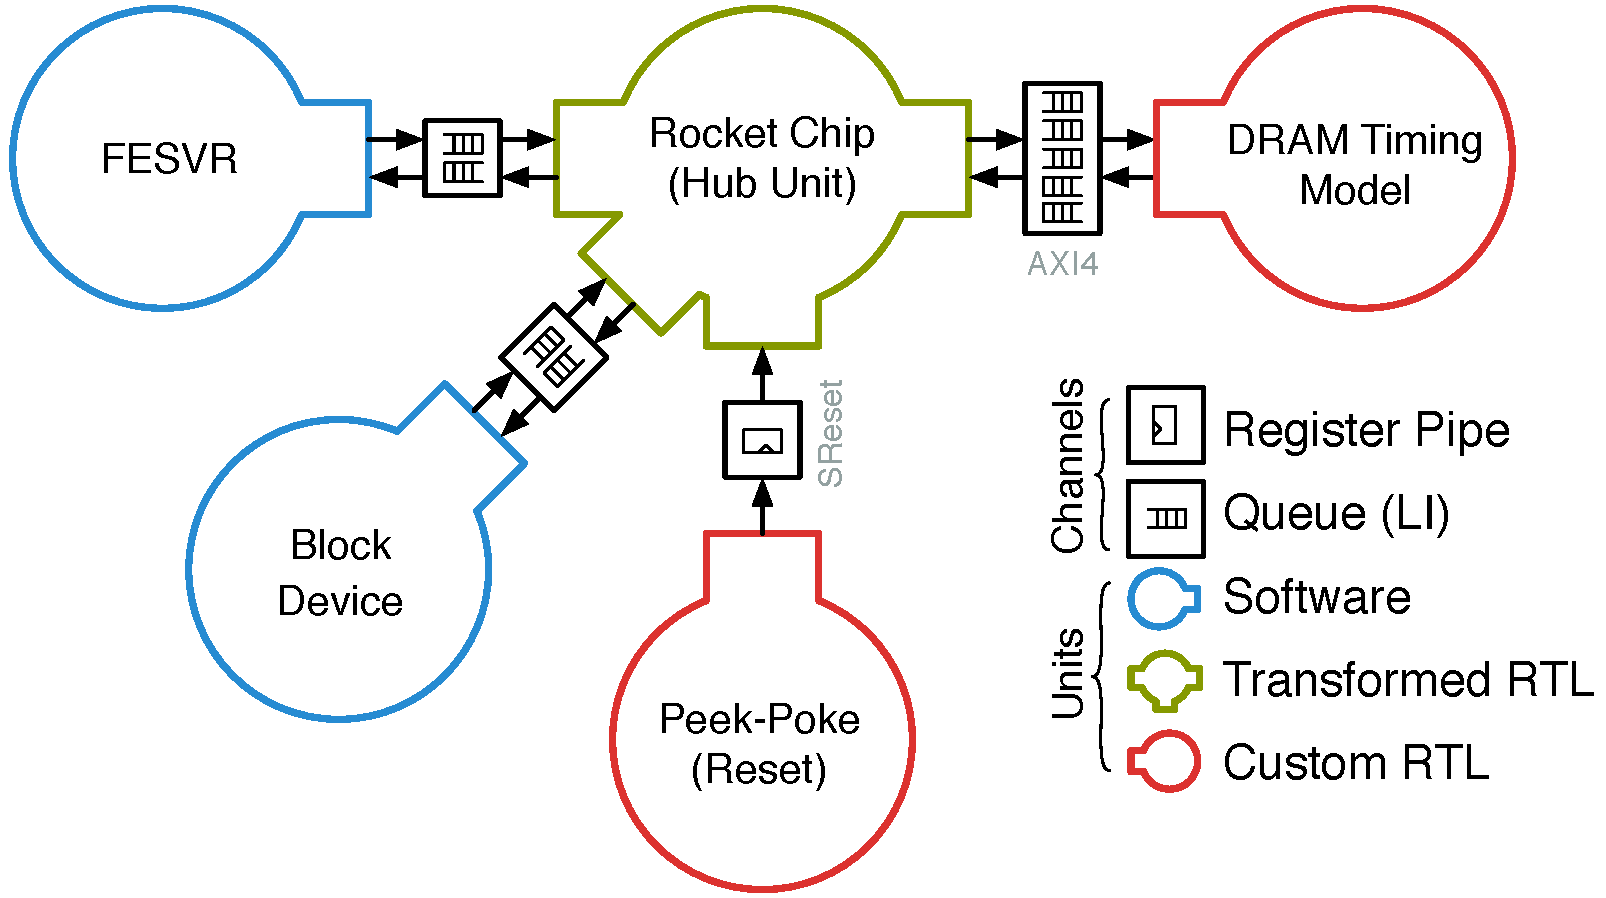
\includegraphics[width=0.9\textwidth]{figures/rocket-target-graph.pdf}
    % graffle2pdf -c rocket-target-graph midas-graphics/graffle/masters-target.graffle figures/rocket-target-graph.pdf
    \caption{The graph of a typical Rocket-Chip-derived system.}
    \label{fig:rocket-target-graph}
\end{figure}

\begin{figure}
    \centering
    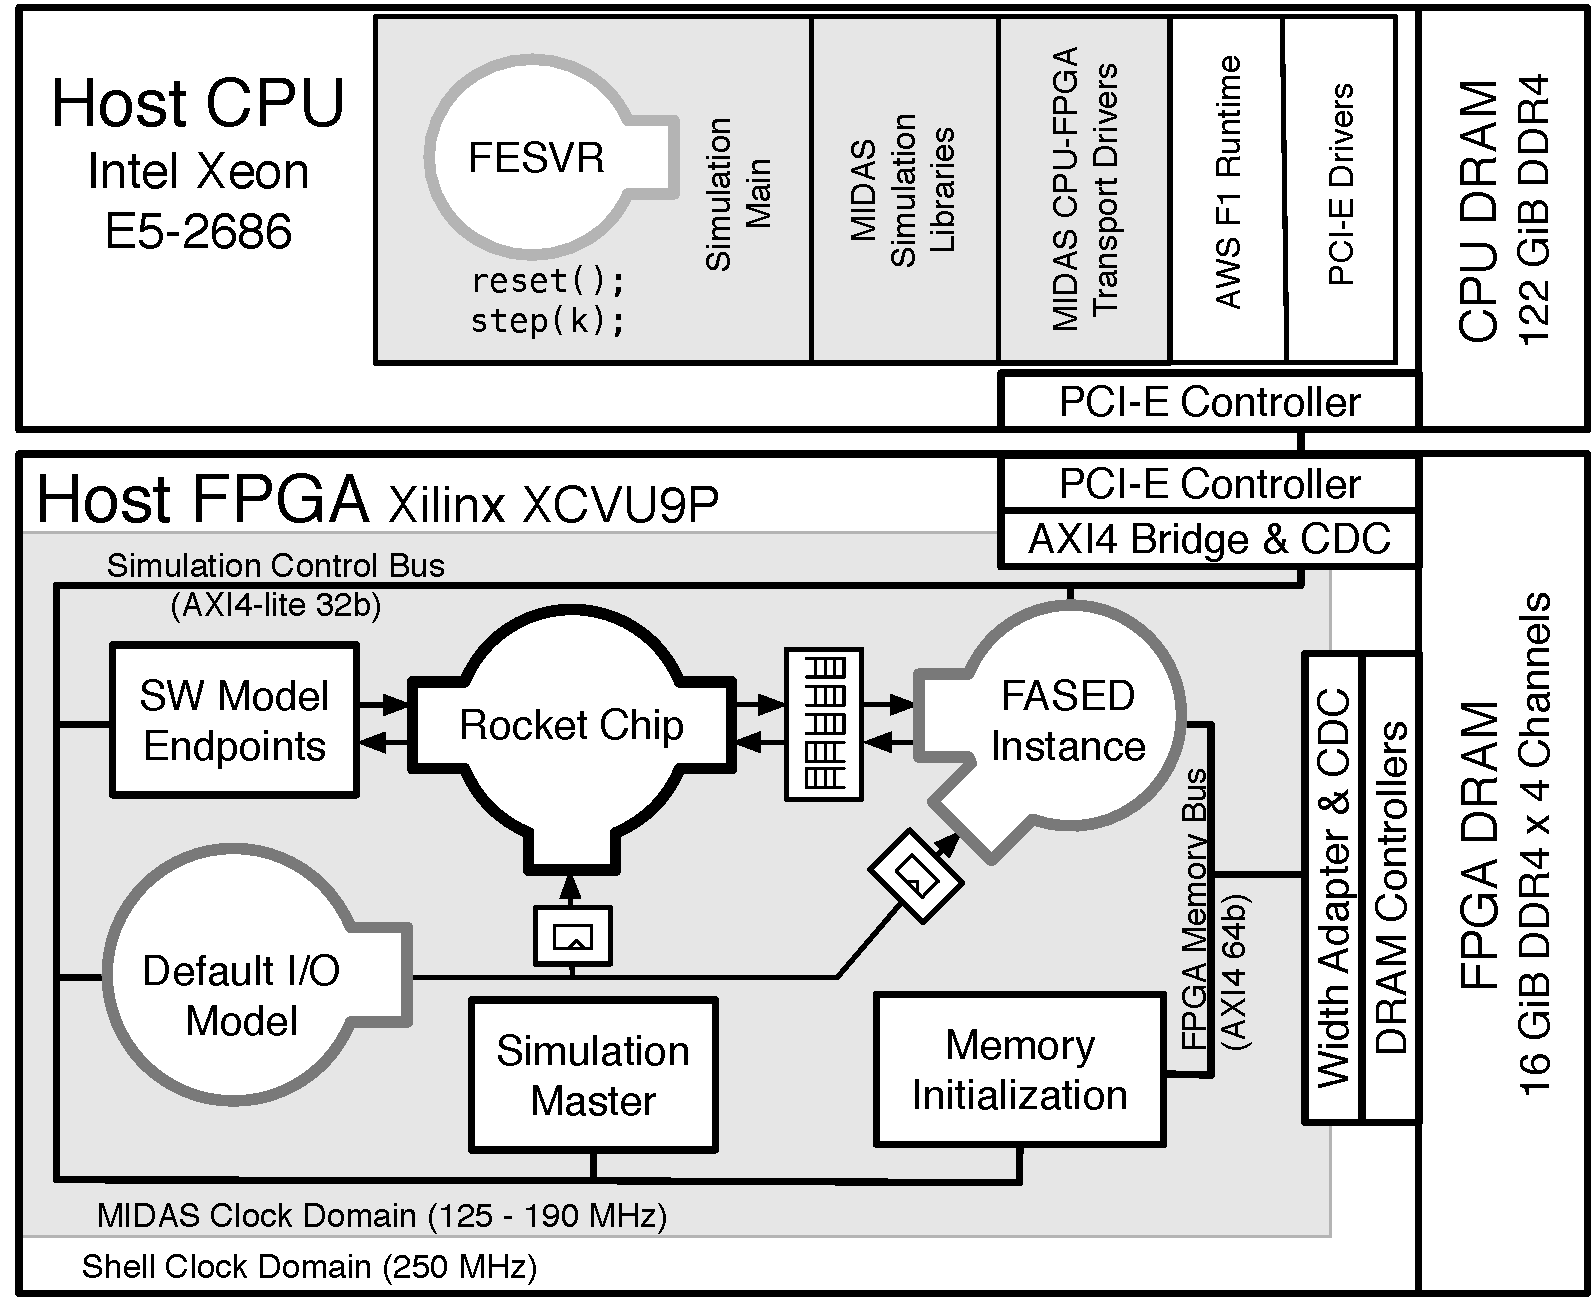
\includegraphics[width=0.9\textwidth]{figures/mapped-simulator-f1.pdf}
    % graffle2pdf -c f1 midas-graphics/graffle/mapped-simulator.graffle figures/mapped-simulator-f1.pdf
    \caption{An example simulator mapped to and EC2 F1 host.}
    \label{fig:mapped-simulator-f1}
\end{figure}


\subsection{Endpoint Units}

Topological position aside, endpoint units differ from the hub in that they are not transformed from ASIC
RTL and instead are written by hand, and thus, not exact models of the desired target system.
Endpoints consist of an \emph{endpoint module}, which resides on the FPGA and drives the channels bound to the hub unit, and an
\emph{endpoint driver}, which is linked into the main simulation driver and hosted on a CPU.
Even the purest "CPU-hosted" units require an endpoint driver that
implements transport for token streams moving on and off the
FPGA\footnote{FireSim stitched together larger targets by adding software units
to represent parts of the network. These were hosted purely on a CPU, often
with no FPGA attached.} Similarly, FPGA-hosted models tend to have a driver
that is reponsible for configuring the FPGA-hosted piece of the unit, and for
polling FPGA-hosted instrumentation.

Endpoints can leverage three types of host resources:

\begin{enumerate}
\item CPU-mastered MMIO. Here, modules expose 32-bit registers that can be
    written to and read from the driver. This is typically used to expose
    configuration  parameters that the driver initializes before simulation
    commences, and to expose instrumentation that can be polled during
    simulation. Generally, MMIO cannot provide enough bandwidth to support transporting token streams,
    for low-bandwidth, loosely coupled endpoint it can also be used to pass transaction-level tokens.
    The endpoints for UART and the FireSim block device do this.

\item CPU-mastered DMA. To support moving complete token streams, endpoints can
    bind to CPU-mastered DMA. Here endpoint modules expose hardware FIFOs to the DMA bus to which the driver
    can make bulk (up to 4192KB) reads and writes. If the endpoint is not closely coupled
    to the hub, token transport can be overlapped with simulator execution: the NIC endpoint relies on this
    provide good FMR in networked simulations~\cite{FireSim}. CPU-mastered DMA is also used 
    to drain token streams from instrumentation endpoints. Since these endpoints do not drive
    tokens back to the hub, it is only necessary to provide sufficient DMA read-bandwidth to achieve good FMR.
    Examples of this include the synthesized printf endpoint and the TracerV
    RISC-V instruction trace collection endpoint.

\item FPGA DRAM. Some units require more local storage than FPGA fabric can
    provide, but cannot afford the round trip latency of using CPU memory or
    disk. MIDAS provides a simple means to let endpoints drive the FPGA
    DRAM memory system.  MIDAS's memory timing models, both those described
    in the CARRV publication~\cite{MIDAS} and later by FASED~\cite{FASED},
    use FPGA DRAM as a backing store for a timing model that's implemented
    in FPGA fabric.
\end{enumerate}

Endpoint drivers interact with their associated module using four methods
exposed by the main simulation driver: \texttt{simif::read} and
\text{simif::write} drive CPU-mastered MMIO; \texttt{simif::pull} and
\texttt{simif::push} are used to drive CPU-mastered DMA.

\subsection{Simulation Driver}

The simulation driver is written in C++ and instantiates an endpoint driver class for each endpoint
in the system. Once the FPGA has been flashed, the driver can be launched.
Simulation proceeds in three phases:

\begin{enumerate}
    \item Initialization. This provides a window for endpoint drivers to do DMA
        and MMIO before the simulation commences.  Here the driver optionally
        zeros-out or intializes FPGA DRAM, before calling each endpoint
        driver's \texttt{init} method, which sets up configuration registers on
        the FPGA that may control timing parameters or instrumentation modes.

    \item Execution. Here the driver invokes each endpoint's \texttt{tick}
        method in a tight loop, in round-robin order.  Drivers issue MMIO and
        DMA requests attempting to make forward progress without blocking.

    \item Teardown. Simulation ends once any endpoint driver calls for
        termination. The driver calls each endpoint's \texttt{finish} method,
        which gives the endpoint a final opportunity to do FPGA DMA and MMIO. This
        typically includes reading final FPGA-hosted intrumentation values and commiting simulation output to disk.
\end{enumerate}


\subsection{Time Control}
After FPGA programming and reset, channels are ready to produce initial tokens and thus units are free
to begin executing. Generally, endpoints that require
configuration wait for an MMIO register to be set during the driver's
intialization phase before acting on token streams. In the absence of
user-provided endpoints, MIDAS prevents the hub model from free-running by
mandating that all target designs have a synchronous reset that is driven
by a special \emph{peek-poke} endpoint. The peek-poke endpoint ties off all
unnconnected I/O on the target to memory-mapped registers
that can be driven to specific constants during initialization, or
periodically changed during simulation. The driver can then "step" the hub
by controlling the emission of reset tokens by the peek-poke endpoint.
Unlike for other endpoints, channels between the peek-poke endpoint and hub
are the only channels that are wire-type by default: enqueuing a $k$ reset
tokens permits the hub to advance no further than cycle $k$.

During simulation teardown, the simulator estimates the number of cycles simulated by
reporting the number of reset tokens enqueued by the endpoint. In practise,
the hub may not have drained all tokens in the reset channel (it is in the
past relative to the peek-poke endpoint), and additionally, other endpoints
connected to the hub may be relatively more or less advanced in simulation
time due to the distributed nature of the simulator.

\subsection{Using MIDAS: Generator Side Integration}

MIDAS functions by providing an alternate generation flow for a Chisel
generator.  In their Scala application, the user lazily instantiates their
module class and calls out to chisel elaboration as they normally would.
This produces a FIRRTL circuit and annotations for what will become the hub
model.  Typically the lifetime of a chisel module class ends after
elaboration, however the lazy reference to the class allows the user to
extract the Scala types and names of the I/O interfaces of the top-level
module after elaboration. This is critical as MIDAS determines how to bind
endpoints to the hub unit by querying a user-provided map of Chisel type to
endpoint module for each of the extracted I/O interfaces. Finally, the user
invokes the compiler, passing the FIRRTL circuit and annotations, the
extracted I/O list, separate lists of FIRRTL transforms to run on the
elaborated RTL and then the complete simulator, and an implicit parameters
instance which provides the aforementioned map and set switches to control
various stages of the compiler.

\subsection{MIDAS Compiler Flow}

\begin{figure}
    \centering
    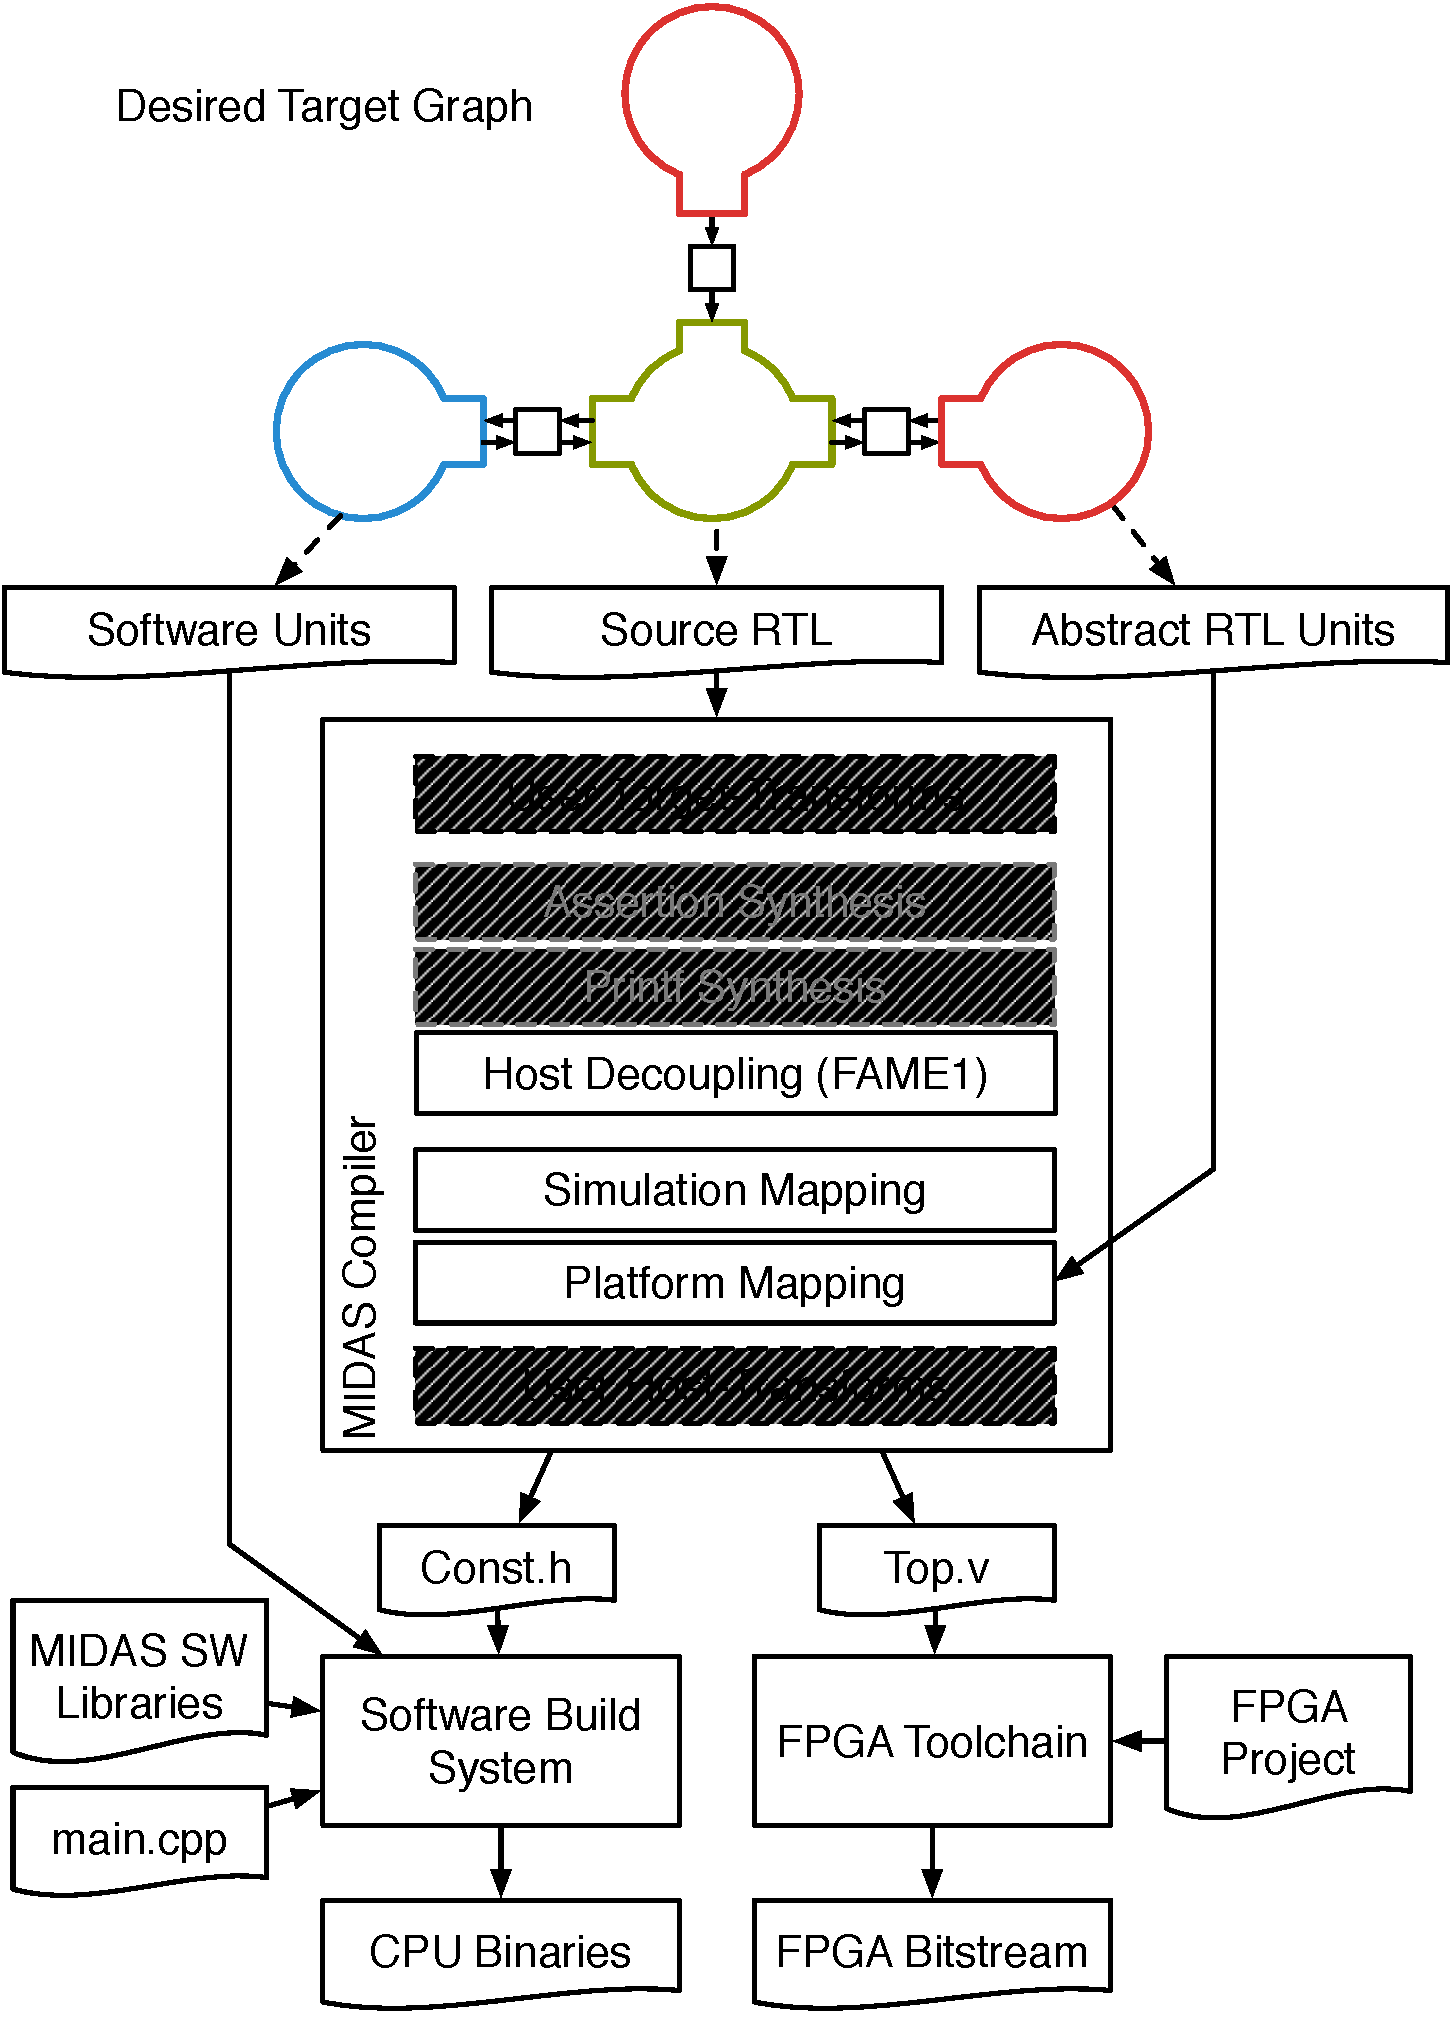
\includegraphics[width=0.9\textwidth]{figures/midas-flow.pdf}
    % graffle2pdf -c midas-flow midas-graphics/graffle/toolchain.graffle figures/midas-flow.pdf
    \caption{The end-to-end flow of a MIDAS compilation.}
    \label{fig:midas-flow}
\end{figure}

We show the flow the MIDAS compiler in Figure~\ref{fig:midas-flow}.

Before running core transformations, MIDAS schedules user-provided target transforms.
In FireSim, dedicated passes to remove unsupported verilog black-boxes and
replace asynchronously reset registers synchronously reset ones.

Next MIDAS runs instrumentation transformations, including printf synthesis
and assertion synthesis~(these were initially presented in DESSERT~\cite{DESSERT}), if they have been requested by the user. These
transformations "synthesize" \texttt{printf} and \texttt{stop} FIRRTL IR
nodes by replacing them with a connections to new top-level outputs. Stops are
replaced with a boolean that is asserted on cycles the stop condition is asserted. Similarly, printfs are replaced with an aggregate that contains
the arguments for the printf's format string and an enable indicating the
printf would trigger on that cycle. Like the other I/O interfaces, these new outputs will be bound to a single asssertion
and printf endpoint later in the compiler.

Now MIDAS runs its FAME-1 transform, transforming the RTL (an SSM) into a
unit.  MIDAS converts the SSM into a patient SSM by injecting clock-enables
on all registers (this introduces a 2:1 mux on register inputs) and by
masking FIRRTL memory write enables. The transform divides and maps the
SSM's I/Os into token ports by recursing through their corresponding Chisel types.
Decoupled interfaces~(latency-insensitivity interfaces that use a ready-valid
handshake) are split into a forward and reverse port, all other
interface types are given a seperate port per leaf-element.  With the I/Os
mapped into unit ports, the transform drives \texttt{fire} with the
conjuction of all inputs' valid and all outputs ports' ready. The resulting
unit is a direct implementation of an APort Network node.

To complete the simulator, MIDAS then wraps the hub unit with two layers of Chisel-generated modules.
In \emph{Simulation Mapping}, MIDAS again recursively walks the chisel-types of the I/O, this time
to generate the channel implementations.
Wire and pipe-type channels are implemented using a queue whose
payload is the underlying hardware type of the target interface. The endpoint and hub can decouple
as many cycles as these queues are deep.  Queue-type channels use a more sophisticated implementation
that drives forward and reverse token streams. The queue channel
implementation allows endpoint and hub to decouple under more specific runtime conditions~(for example,
while a queue is not full it can continue to accept forward tokens and produce reverse tokens on its the producer side
of the queue.

In \emph{Host Platform Mapping}, MIDAS recursively walks the chisel-types
of the I/O a final time, here it attempts to find a provided endpiont for
each type using the Endpoint Map. If the map is defined on that type, MIDAS
instantiates the endpoint module, and connects its tokenized host port to the freshly
generated channels. All remaining unbound interfaces are then bound to the
peek poke endpoint. Once all endpoints have been elaborated, it binds their
MMIO interfaces and DMA interfaces, if present, to the simulation control
and DMA buses, respectively, using a $1:N$ AXI4 arbiter. Memory timing
models have their host-memory interface driven to DRAM memory interfaces,
this time through an $M+1:N$ AXI4 crossbar, where $M$ is the number of
target memory models and $N$ is the number of host memory channels. The
extra master port is driven by the loadmem unit, which bridges the
simulation control bus and memory bus and gives the driver the means to
read and write to FPGA DRAM. The parameters of the host platform,
specifically the width of these buses, and the number of memory channels
are defined in the user-provided parameters instance. At this point MIDAS,
generates a C++ header with all of the driver-required metadata for the
simulator. Each endpoint module emits a fragment which contains its allocated MMIO and
DMA addresses, as well as additional constructor parameters required by its
endpoint driver.

In a final step before verilog emission, MIDAS schedules the user's
\emph{host transforms}.  This provides a means to programmatically modify simulator RTL to further
customize it for a host platform. In FireSim, the \texttt{AutoILA}
transform is run here to plumb out annotated signals to a Xilinx Integrated
Logic Analyzer (ILA), which is required in for EC2 F1 hosts due to
restrictions in Amazon's compilation flow. Finally, the FIRRTL optimization passes are run
and the simulator verilog is emitted, and the compiler terminates.

At this point, the user links the generated header into the simulation
main, and compiles the generated verilog into a FPGA shell project.
FireSim's build system automates much of this, and provides an FPGA shell
project for EC2 F1 FPGAs. FireSim's manager \texttt{buildafi} will batch
out bitstream builds to remote hosts on EC2. Similary, its
\texttt{infrasetup} process compiles the simulation driver, in addition to
preforming the other required tasks to prepare for running a simulation
such as flashing the FPGA.

\section{Reviewing MIDAS's Limitations}

At the end of the previous chapter, we indentified two limitations with MIDAS
that we aimed to address in Golden Gate. The first was that it did little to
optimize FPGA resource utilization, precluding the its use for systems of
non-trivial scale. We made our first attempt at addressing this in Golden Gate
in its eponymous ICCAD 2019 publication~\cite{Golden Gate}, by switching to a
LI-BDN formalism, and building in compiler support to indentify, and extract
target submodules in the target design, and then later replacing with
optimized primitive LI-BDN implementations. We expand on the design of this initial version of Golden Gate
in the next chapter~(Chapter~\ref{sec:golden-gate}). Continued work on FAME-compiler-driven optimizations
is the subject of Albert Magyar's Dissertation.

Tackling the second challenge -- supporting realistic simulations of systems
with multiple clock domains, and asynchronous reset -- will take yet another
rethinking as the SSM-assumption fundamental to LI-BDN and APort Network
formalisms no longer applies. In Chapter~\ref{sec:static-multiclock}, we
describe a simple extension to Golden Gate to support multiple target clock
domains under the assumption that they are fixed and rationally related to one another.
Here, we can still treat the target as synchronous -- but to an
artifically fast simulation clock whose frequency is the least-common multiple
of requested clocks. This assumption permits simulators remain implicitly
timestamped.

To build a true emulation environment capable of simulating a broad class of
asynchronous events that manifest in realistic SoCs, including asynchronous
reset and clock generation and switching, and certain non-idealities like clock
drift and jitter , we lift the rational clock assumption and introduce explicit
timestamping into a sub-graph of simulator. Our intial implementation,
described in Chapter~\ref{sec:dynamic-multiclock}, uses a hardware
implementation of the Chandy-Misra-Bryant algorithm to avoid
deadlock.  This explicitly timekept portion of the graph co-exists with SSM
optimizations which can be applied locally to parts of the design where the SSM
assumption holds.

%We considered a few possibilities such as leaning on the endpoint system and
%user modifications to the target RTL, or using specialized transformations to
%implement optimizations as modifications to the hub model.
%We had the following objectives:
%
%\being{itemize}
%\item Minimize user modification to the ASIC RTL.
%\item Make it possible to optimize blocks that may be combinationally coupled to some part of the hub.
%\item Provide a mechanism to rigorously verify the resulting simulator.
%\end{itemize}
%
%
%Ultimately, it was clear that the next compiler needed a generalized
%mechanism to identify and perform optimizations. To make it easier to
%implement optimizations, Golden Gate uses the LI-BDN target formalism,
%removing the explicit need for channels. We acknowledge that forcing
%optimizations to apply only at registered boundaries between units -- a
%requirement of a channel-bootstrapped formalism -- would produce simulators
%with better FMR, this would add complexity to passes in the compiler and
%might make some optimizations infesible.  We also note that these sorts of
%optimizations not fundamentally precluded by LI-BDN: when an edge between
%two LPs is driven by an output port with no combinational dependency on an
%input, it may be possible to implement that edge using flow queue to save a
%cycle of transmission latency.
%
%Moving to an LI-BDN formalism resolves a number of other modeling
%challenges MIDAS users face.  Requiring that non-wire-channels be injected
%between endpoints and the hub unit was too restrictive in some cases where
%the user wishes to model a combinational path that propagated through the
%endpoint. Another challenge was defining the reset semantics of these
%stateful channels.  MIDAS relies on FPGA programming to properly initialize
%these channels, however they are not held in target reset  during
%simulation: it is purely coincidental that the hub model does not
%spuriously enqueue target data into queue-type channels while parts of the
%hub are under target reset. For a time, MIDAS would broadcast target reset
%tokens to channels and endpoints, but too is fraught as resets driving
%registers in the hub maybe different from this special-cased global reset.
%Instead of requiring that user specify this reset for each channel, LI-BDN
%can sidestep these issues entire by removing the need for stateful
%channels, allowing the compiler to assume fewer things about target.

